\section{实验结果}

\subsection{\(\ce{Fe(OH)3}\)溶液的热透析纯化}

记录\(\ce{Fe(OH)3}\)溶液的热透析纯化过程的时间,并使用$\ce{KSCN}$检测$\ce{Fe^3+}$,使用$\ce{AgNO3}$检测$\ce{Cl-}$,当离子基本无法检出时,记录透析液的电导,最终测定溶胶的电导。其中,“+”表示检出该离子、“-”表示未检出该离子。

\begin{table}[htbp]
\centering
\bicaption{Fe(OH)$_3$ 溶胶透析过程表}{Table of Dialysis Process for Fe(OH)$_3$ Sol}
\begin{tabular}{cccccc}
\toprule
编号 & 透析时长 $t$ / min & $\ce{Fe^3+}$ 检测 & $\ce{Cl-}$ 检测 & 透析液电导 / $\mu$S$\cdot$cm$^{-1}$ & 溶胶电导 / $\mu$S$\cdot$cm$^{-1}$ \\
\midrule
1 & 11 & + & + & & \\
2 & 13 & + & + & & \\
3 & 15 & - & + & & \\
4 & 15 & - & + & & \\
5 & 15 & - & + & & \\
6 & 19 & - & + & & \\
7 & 16 & - & - & 231.2 & \\
8 & 30 & - & - & 70.7 & \\
9 & 30 & - & - & 22.8 & \\
10 & 15 & - & - & 8.9 & 170.5 \\
\bottomrule
\end{tabular}
\label{tab:1}
\end{table}

\subsection{电极间距测量}

用软尺沿电泳管的中心线测量两电极间的距离 $l$,重复测量三次,结果如表 \ref{tab:3} 所示。
\begin{table}[htbp]
\centering
\bicaption{两电极间距离测量数据}{Measurement Data of Distance Between Two Electrodes}
\begin{tabular}{cccc}
\toprule
编号 &  1 & 2 & 3 \\
\midrule
$l / \mathrm{cm}$ & 22.50 & 22.20 & 22.75 \\
\bottomrule
\end{tabular}
\label{tab:3}
\end{table}

根据表 \ref{tab:3},使用 numpy 求得其均值与标准差为
\begin{gather*}
    \bar{l} = 22.48,\ \sigma_l = 0.22\\
    \therefore l=(22.48 \pm 0.22) \mathrm{cm}
\end{gather*}

\subsection{溶胶电泳实验结果}

在 \(\ce{Fe(OH)3}\) 溶胶电泳实验过程中,记录正负两极的界面位置随时间的变化,结果如表 \ref{tab:2} 所示,其中 $t$ 为电泳实验进行的时间,$h{(-)}$、$\Delta h{(-)}$ 为溶胶在负极界面位置与移动距离,$h{(+)}$、$\Delta h{(+)}$ 为溶胶在正极极界面位置与移动距离。

\begin{table}[htbp]
\centering
\bicaption{\(\ce{Fe(OH)3}\) 溶胶电泳界面迁移距离的计算结果}{Calculation Result of Migration Distance of \(\ce{Fe(OH)3}\) Sol Electrophoresis Interface}
\begin{tabular}{ccccc}
\toprule
$\mathrm{t} / \mathrm{s}$ & $h_{(-)} / \mathrm{cm}$ & $\Delta h_{(-)} / \mathrm{cm}$ & $h_{(+)} / \mathrm{cm}$ & $\Delta h_{(+)} / \mathrm{cm}$ \\
\midrule
0 & 3.95 & 0.00 & 3.90 & 0.00 \\
59 & 4.04 & 0.09 & 3.79 & 0.11 \\
116 & 4.14 & 0.19 & 3.69 & 0.21 \\
179 & 4.22 & 0.27 & 3.58 & 0.32 \\
248 & 4.33 & 0.38 & 3.43 & 0.47 \\
319 & 4.47 & 0.52 & 3.43 & 0.47 \\
383 & 4.61 & 0.66 & 3.23 & 0.67 \\
433 & 4.66 & 0.71 & 3.01 & 0.89 \\
503 & 4.74 & 0.79 & 3.10 & 0.80 \\
571 & 4.93 & 0.98 & 2.84 & 1.06 \\
\bottomrule
\end{tabular}
\label{tab:2}
\end{table}

在 \(\ce{Fe(OH)3}\) 溶胶电泳实验进行过程中,由于氢氧化铁胶粒带正电,向负极迁移,与观察到的形管负极一侧上升,正极一侧下降相吻合。观察界面状态以及电极表面的变化。随着电泳实验的进行,两侧电极表面有少量气泡产生,右侧比左侧产生的气泡更多;左侧正极界面在下降过程中越来越模糊,这是因为正极发生氧化反应析出氧气,生成$\ce{H+}$将溶胶逐渐溶解;而右侧界面在上升过程中越来越清晰,且产生少量粉黄色模糊状沉淀,这是因为负极发生还原反应析出氢气,生成$\ce{OH-}$与溶胶反应形成\(\ce{Fe(OH)3}\)沉淀。

使用python matplotlab,将表 \ref{tab:2} 的数据作图,使用python scipy.stats.lingress 将界面移动距离与电泳时间做线性回归,如图 \ref{fig:1},线性回归的结果如表 \ref{tab:4}。

\begin{figure}[htbp]
    \centering
    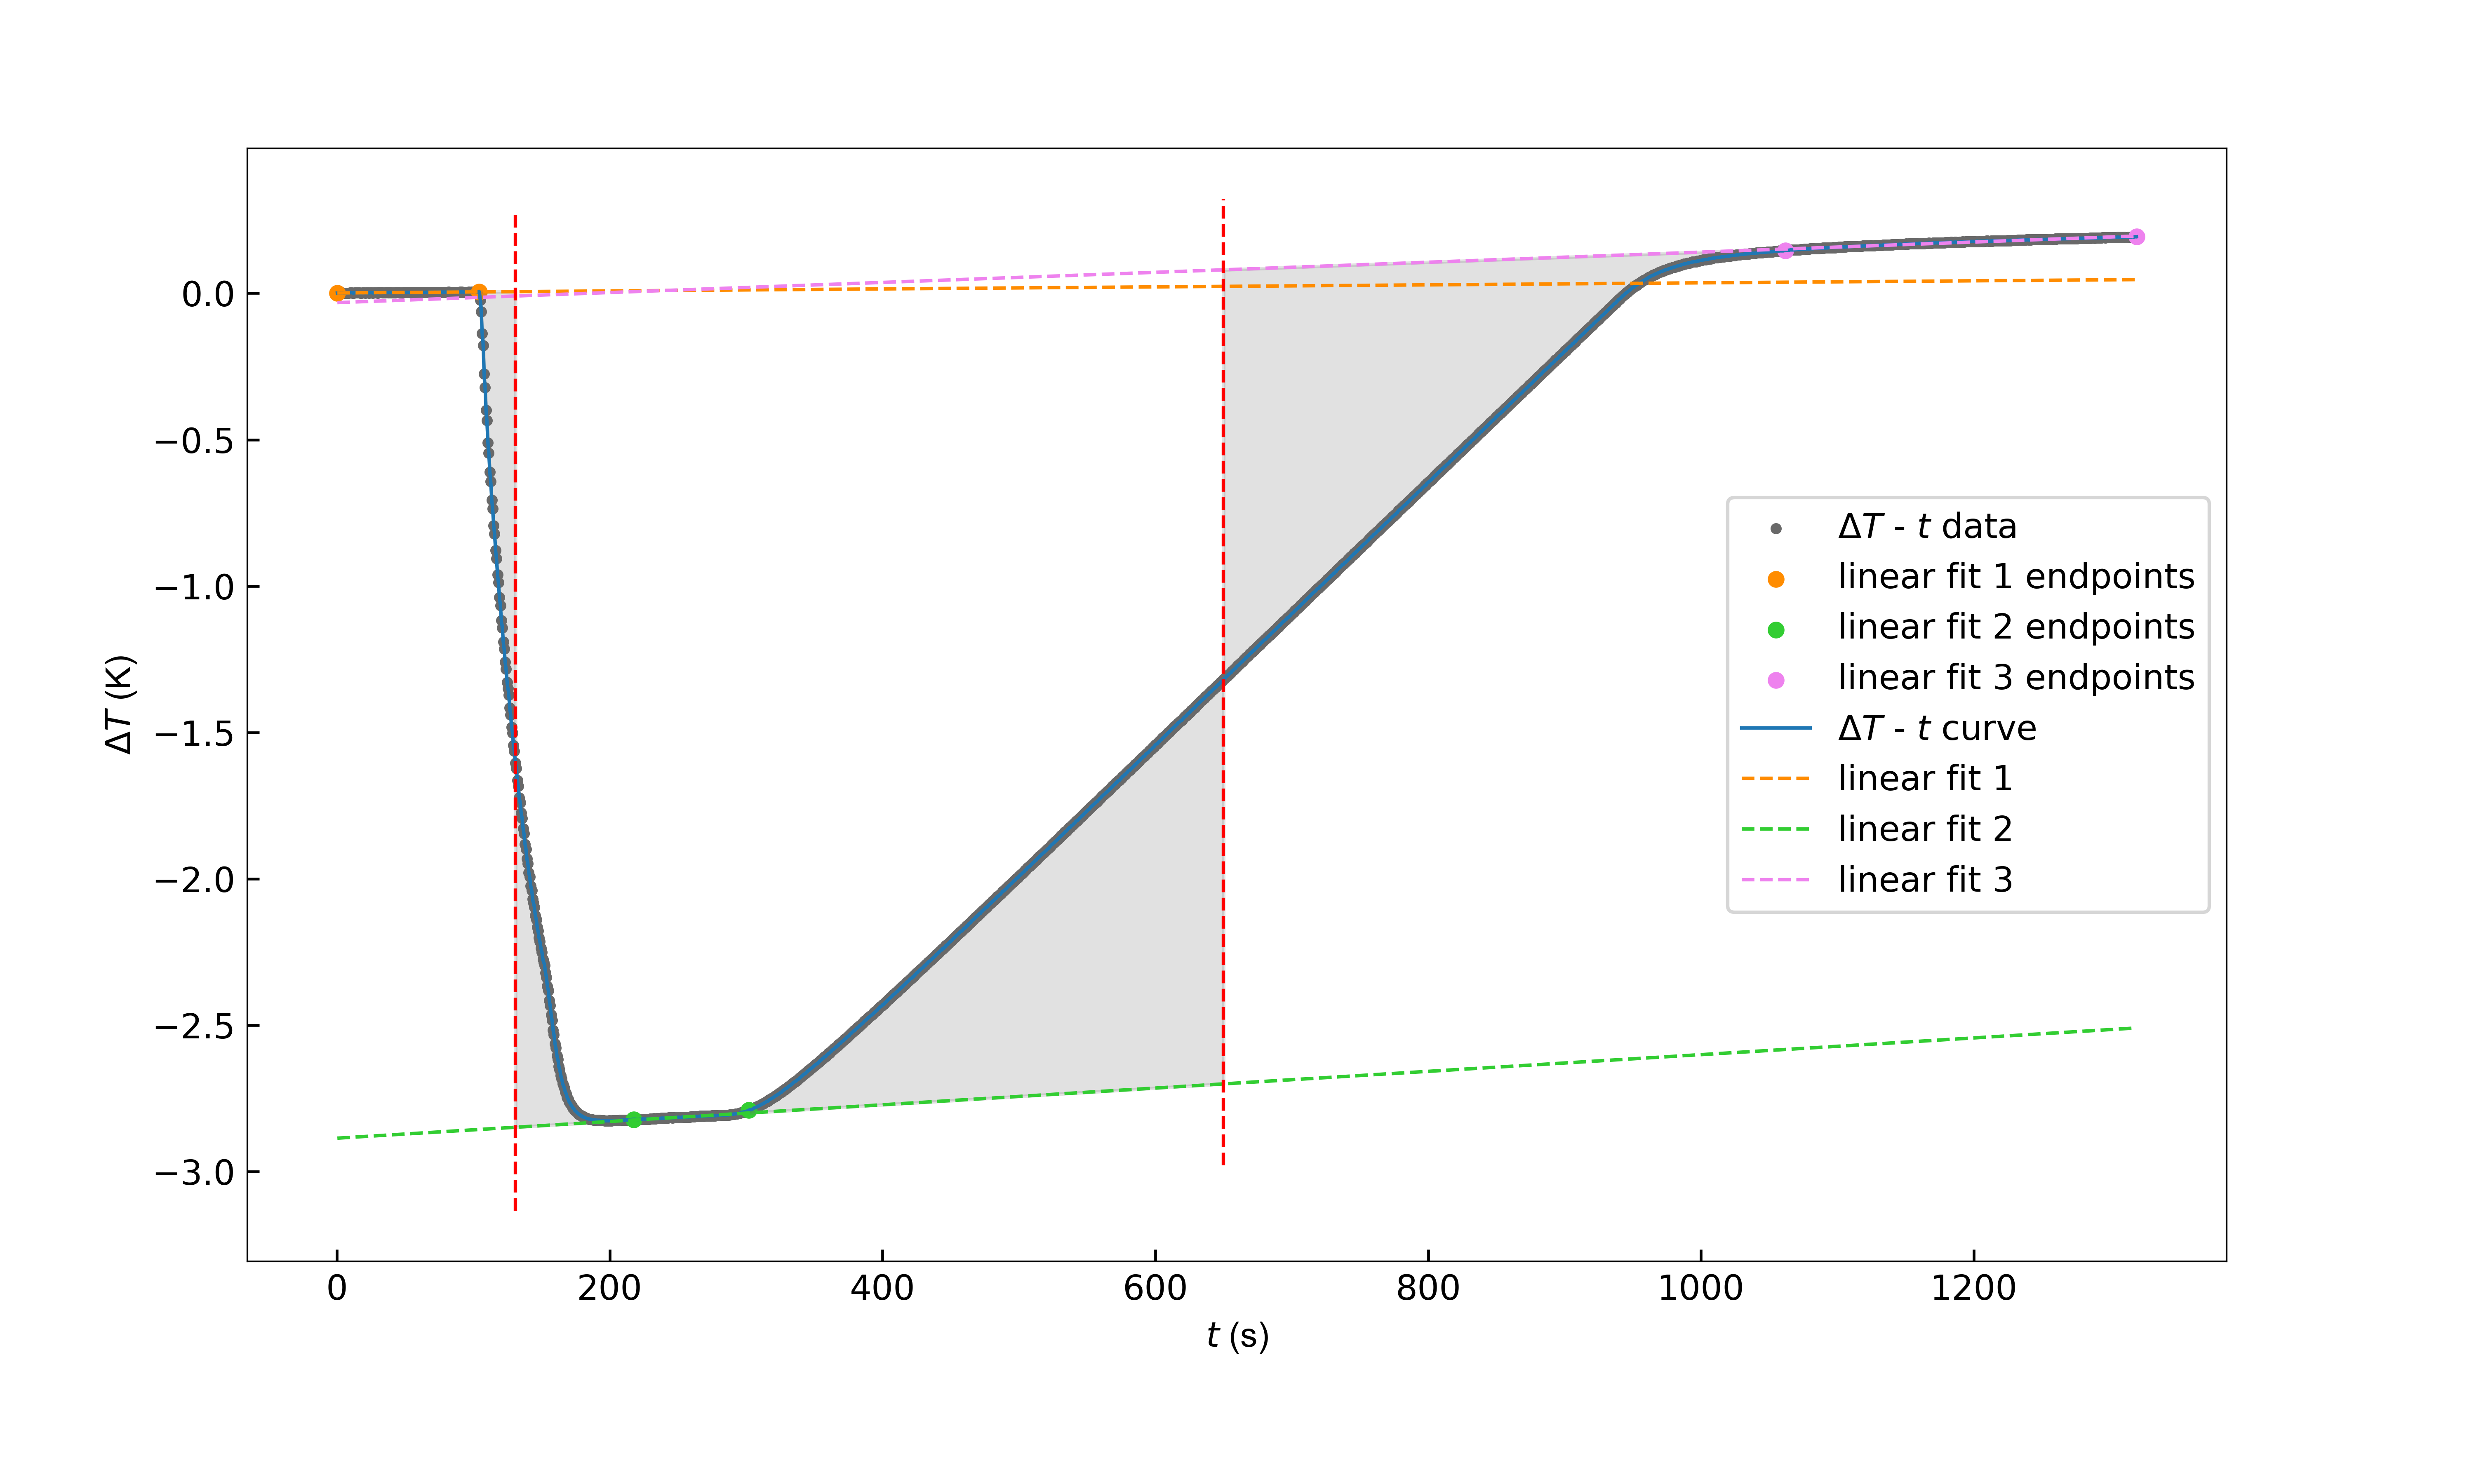
\includegraphics[width=.8\textwidth]{figures/1.png}
    \bicaption{\(\ce{Fe(OH)3}\) 溶胶电泳时间界面迁移距离关系图}{Relat. Graph of Interface Migration Distance over Time in Electrophoresis of \(\ce{Fe(OH)3}\) Sol}
    \label{fig:1}
\end{figure}
\begin{table}[htbp]
\centering
\bicaption{电极迁移距离与电泳时间的线性回归结果}{Linear Regression Results of Electrode Migration Distance and Electrophoresis Time}
\begin{tabular}{cccccc}
\toprule
电极 & $v / \mathrm{cm \cdot s}^{-1}$ & $\sigma_v / \mathrm{cm \cdot s}^{-1}$ & $b / \mathrm{cm}$ & $\sigma_b / \mathrm{cm}$ & $R^2$ \\
\midrule
(-) & 0.00168 & 0.00004 & -0.01275 & 0.00003 & 0.99481 \\
(+) & 0.00179 & 0.00012 & -0.00197 & 0.00007 & 0.96763 \\
\bottomrule
\end{tabular}
\label{tab:4}
\end{table}

由图 \ref{tab:4} 可以发现,由于负极界面清晰易于观察,其拟合线性程度很好,而正极由于溶胶溶解界面难以观察,线性程度远不如负极的结果。
计算两侧界面迁移的平均速度
$$
v=\frac{v(-)+v(+)}{2}=0.00172 \mathrm{~cm} \cdot \mathrm{s}^{-1}
$$
界面迁移速度的不确定度
$$
\sigma_v=\sqrt{\sigma_{v(-)}^2+\sigma_{v(+)}^2}=0.00012 \mathrm{~cm} \cdot \mathrm{s}^{-1}
$$

\subsection{溶胶电动电势的计算}

使用以下公式计算 \(\ce{Fe(OH)3}\) 溶胶的电动电势 $\zeta$,:
$$
\zeta = \frac{\eta v l}{\varphi \varepsilon_r \varepsilon_0}
$$
其中,两电极间距离 $l = (22.48 \pm 0.22) \, \mathrm{cm}$,界面迁移的平均速度 $v = (0.00172 \pm 0.00012) \, \mathrm{cm} \cdot \mathrm{s}^{-1}$,两电极间的电势差 $\varphi = (100\pm 1) \, \mathrm{V}$。根据\textit{CRC Handbook of Chemistry and Physics}\cite{haynes2016crc}真空介电常数 $\varepsilon_0 = 8.8542 \times 10^{-12} \, \mathrm{F} \cdot \mathrm{m}^{-1}$,在 $20^\circ\mathrm{C}$ 时水的相对介电常数 $\varepsilon_r = 80.10$。依据《物理化学实验 (第四版)》附录表 D.4-15\cite{pku2002physicalchem},当 $t = 17^\circ\mathrm{C}$ 时水的黏度 $\eta = 1.083 \, \mathrm{mPa} \cdot \mathrm{s}$,考虑温度存在 $\pm 1^\circ\mathrm{C}$的波动,根据书中数据假定 $\sigma_\eta=0.004 \mathrm{mPa} \cdot \mathrm{s}$,$\sigma_{\varepsilon_r}=0.03$。

首先计算得到溶胶电动电势:
$$
\zeta = \frac{1.083 \times 10^{-3} \, \mathrm{Pa} \cdot \mathrm{s} \times 0.00172 \, \mathrm{m/s} \times 0.2248 \, \mathrm{m}}{100 \, \mathrm{V} \times 80.10 \times 8.8542 \times 10^{-12} \, \mathrm{F/m}} = 0.05904\mathrm{~V}
$$
求出其不确定度:
$$
\begin{aligned}
\sigma_{\zeta} 
& = \zeta \sqrt{\left(\frac{\sigma_\eta}{\eta}\right)^2+\left(\frac{\sigma_v}{v}\right)^2+\left(\frac{\sigma_l}{l}\right)^2+\left(\frac{\sigma_{\varphi}}{\varphi}\right)^2+\left(\frac{\sigma_{\varepsilon_r}}{\varepsilon_r}\right)^2} \\
& = 0.05904 \sqrt{\left(\frac{0.003 \times 10^{-3}}{1.083 \times 10^{-3}}\right)^2 + \left(\frac{0.00012}{0.00172}\right)^2 + \left(\frac{0.0022}{0.2248}\right)^2 + \left(\frac{1}{100}\right)^2 + \left(\frac{0.03}{80.10}\right)^2}\\
& = 0.0047\mathrm{~V}
\end{aligned}
$$
由此可得, 测算得到的电动电势为 $\zeta=(59 \pm 5) \mathrm{mV}$




















